\section{Implementation}
\label{sec:implementation}

In this section we describe an implementation of the \lloid\ method described
in section \ref{sec:method} suitable for rapid gravitational-wave
searches for compact binary coalescence.  The \lloid\ method requires several
computations that can be completed before the analysis is underway.  Thus
we divide the procedure into two stages 1) an offline planning stage and 2) an
online, low-latency filtering stage.  The offline stage can be done before the
analysis is started and updated asynchronously, whereas the online stage must
keep up with the detector output and produce search results as rapidly as
possible.  In the next two subsections we describe what these stages entail.

\subsection{Planning stage}

The choice of templates and the \SVD\ can be done in
advance and will be valid as long as the detector noise spectrum remains
roughly constant%
\editorial{I'd rather not go into this.}%
.  New templates and the \SVD\ can be computed asynchronously using
updated spectrum estimates as they are available. 

\begin{figure}[htbp]
	\label{fig:tmpltbank}
	\begin{center}
		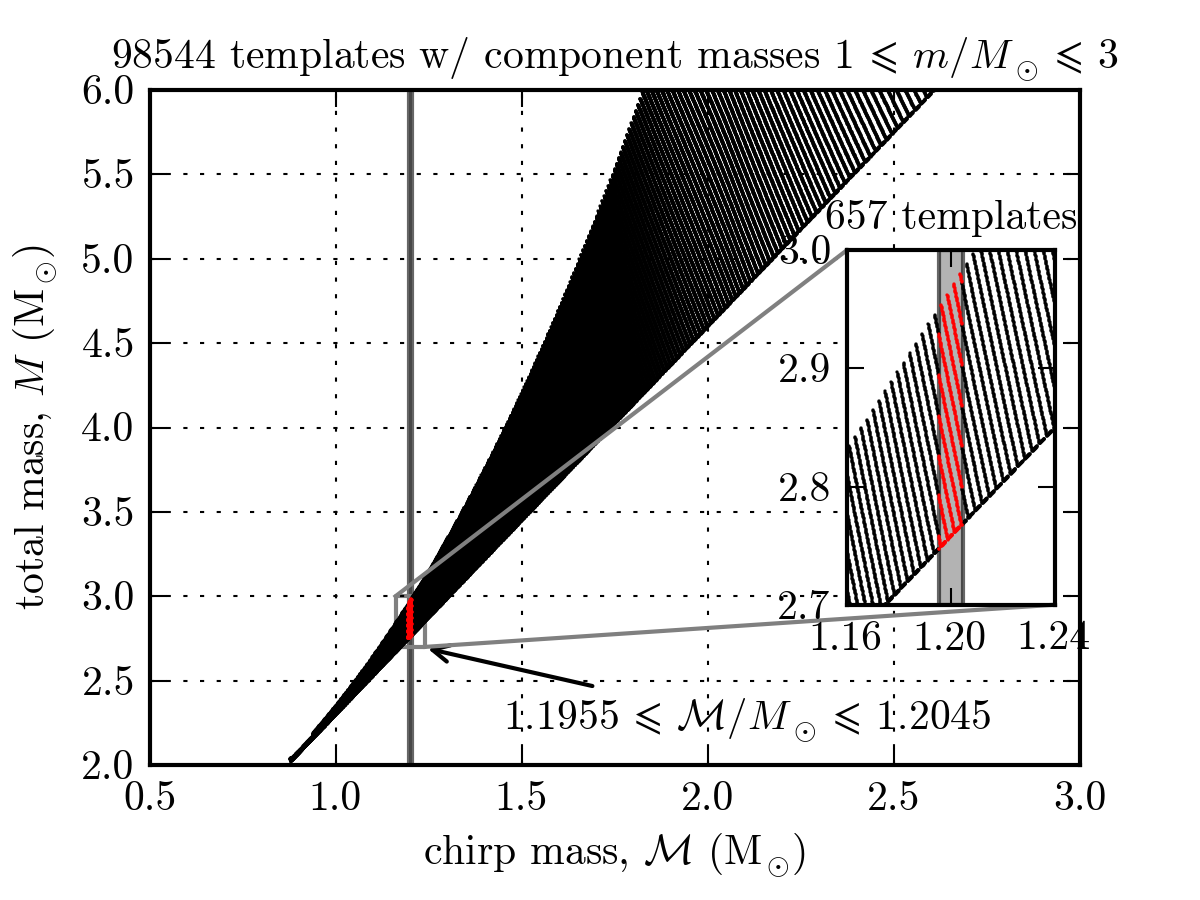
\includegraphics{figures/tmpltbank.png}
		\caption{Placement of template parameters used in this paper.  The template bank consists of 98544 templates with component masses $m_1$, $m_2$, between 1~and~3~$M_\odot$.  We shall design a filter bank to search for a small subset of these template parameters with chirp masses $\mathcal M$ between 1.1955~and~1.2045~$M_\odot$.}
	\end{center}
\end{figure}

\begin{table}
\begin{indented}
\caption{Filter design for these 657 templates.  From left to right, this table shows the sample rate, time interval, number of samples, and number of orthogonal templates for each time slice.  The \SVD{} tolerance is varied from $\left(1-10^{-1}\right)$ to $\left(1-10^{-6}\right)$.}
\item[]\begin{tabular}{rr@{,\,}lc*{6}{r}}
\br
\multicolumn{4}{c}{} &\centre{6}{$\log_{10}$ (1 $-$ \textsc{svd} tolerance)} \\
\ns
\multicolumn{4}{c}{} &\crule{6} \\
$f^s$ (Hz) & $(t^{s+1}$&$t^s]$ (s) & $N^s$ & $-1$ & $-2$ & $-3$ & $-4$ & $-5$ & $-6$ \\
\mr
4096 & (0.5&0] & 2048 & 1 & 4 & 6 & 8 & 10 & 14 \\
512 & (4.5&0.5] & 2048 & 2 & 6 & 8 & 10 & 12 & 16 \\
256 & (12.5&4.5] & 2048 & 2 & 6 & 8 & 10 & 12 & 15 \\
128 & (76.5&12.5] & 8192 & 6 & 20 & 25 & 28 & 30 & 32 \\
64 & (140.5&76.5] & 4096 & 1 & 8 & 15 & 18 & 20 & 22 \\
64 & (268.5&140.5] & 8192 & 1 & 7 & 21 & 25 & 28 & 30 \\
64 & (396.5&268.5] & 8192 & 1 & 1 & 15 & 20 & 23 & 25 \\
32 & (460.5&396.5] & 2048 & 1 & 1 & 3 & 9 & 12 & 14 \\
32 & (588.5&460.5] & 4096 & 1 & 1 & 7 & 16 & 18 & 21 \\
32 & (844.5&588.5] & 8192 & 1 & 1 & 8 & 26 & 30 & 33 \\
32 & (1100.5&844.5] & 8192 & 1 & 1 & 1 & 12 & 20 & 23 \\
\br
\end{tabular}
\end{indented}
\end{table}

The planning stage begins with choosing templates that cover the space of source
parameters with a hexagonal grid~\cite{PhysRevD.76.102004} in order to satisfy
a minimum match criterion.  This assures a prescribed maximum loss in \SNR\
for signals that fall between the chosen templates.  Typically the minimum
match is 0.97 corresponding to a maximum mismatch of 0.03.  Next, the templates
are subdivided into groups of neighbors called \emph{sub-banks} that are
appropriately sized so that each bank can be efficiently handled by a single
computer.  The neighbors are chosen to have comparable chirp mass, which produces
sub-banks with similar time-frequency evolution.  Dividing the source parameter space
into smaller sub-banks reduces the computational cost of the singular value decomposition
and is the approach considered in~\cite{Cannon:2010p10398}.  We choose time
slice boundaries as in equation~\eqref{eq:time-sliced-templates} such that all of the templates within a
sub-bank are sub-critically sampled at progressively lower sample rates.  Next,
the templates within the sub-bank are realized as \fir\ filter
coefficients.  For each time slice, the templates are down-sampled to the
appropriate sample rate.  Finally, the \SVD\ is applied to each time
slice in the sub-bank in order to produce a set of orthogonal \fir\
filters and a reconstruction matrix that maps them back to the original
templates as described in equation~\eqref{eq:svddecomp}.  The down-sampled orthogonal
\fir\ filter coefficients, the reconstruction matrix, and the time slice
boundaries are all saved to disk.

\subsection{Filtering stage}

The \lloid\ algorithm could be used in a true sample-in-sample-out real-time
system.  However, such a system would likely require integration directly into
the data acquisition and storage system of the gravitational-wave
observatories.  A slightly more modest goal is to leverage existing low
latency, but not real-time, signal processing infrastructure in order to
implement the \lloid\ algorithm.  For the near-term this should be a viable 
solution for ultra-low latency searches with $\sim 1s$ intrinsic latency.

We have implemented a prototype of the low-latency filtering stage using an
open-source signal processing environment called \gstreamer\ \cite{gstreamer}.
\gstreamer\ is a vital component of many Linux systems, providing media
playback, authoring, and streaming on devices from cell phones to desktop
computers to streaming media servers.  Given the similarities of
gravitational- wave detector data to audio data it is not surprising that
\gstreamer\ is
useful for our purpose. \gstreamer\ also provides some useful stock signal
processing elements such as resamplers and filters.  We have extended the
\gstreamer\ framework by developing a library called \gstlal{}~\cite{gstlal}
that provides elements for gravitational-wave data-analysis.  Figure
\ref{fig:pipeline} describes schematically how we implement the \lloid\ algorithm
using \gstlal\ and \gstreamer\ components.
%
%
\begin{figure}[htbp]
	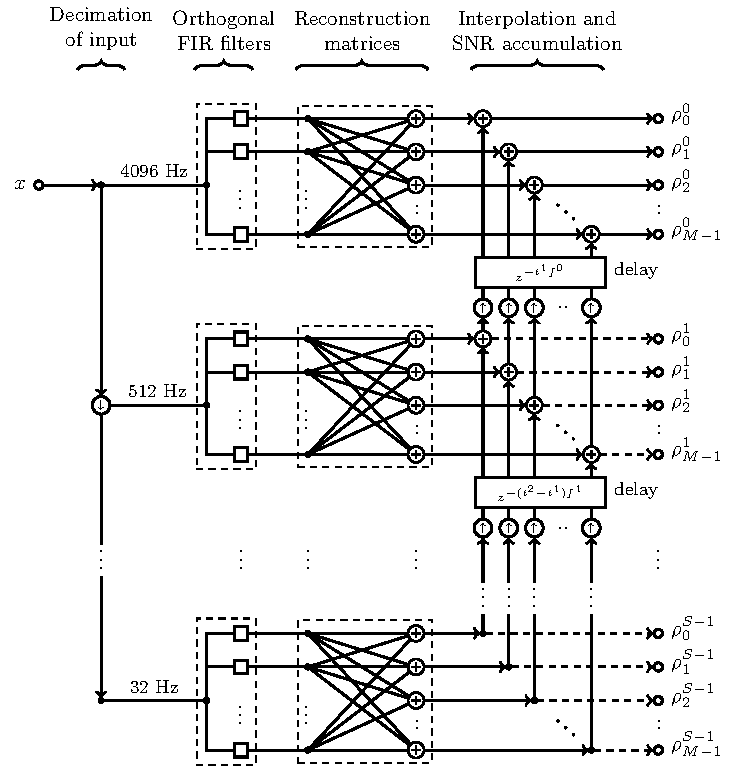
\includegraphics{figures/lloid-diagram.pdf}
	\caption{\label{fig:pipeline} Schematic of \lloid{} pipeline illustrating
signal flow.  Circles with arrows represent interpolation
\protect
\includegraphics{figures/upsample-symbol.pdf} or decimation
\protect
\includegraphics{figures/downsample-symbol.pdf}.  Circles with plus
signs represent summing junctions
\protect
\includegraphics{figures/adder-symbol.pdf}.  Squares
\protect
\includegraphics{figures/fir-symbol.pdf} stand for \fir{} filters.  Sample
rate decreases from the top of the diagram to the bottom.  In this diagram each
time slice contains three \fir\ filters that are linearly combined to produce
four output channels.  In a typical pipeline the number of \fir\ filters is
much less than the number of output channels.}
\end{figure}

The signal flow diagram drawn in figure \ref{fig:pipeline} contains several
distinct stages and parallel branches.  The stages are decimation, filtering
the data against the orthogonal templates, reconstruction of the original template basis, interpolation
and accumulation of the early-warning and final {\SNR}.  We outline the stages
below. 

\subsubsection{Decimation}

First, the sample rate of the whitened detector data is reduced to successively
lower sample rates by decimation.  Decimation involves applying an anti-aliasing
filter to the data, and then down-sampling by deleting samples.  We use a
192-tap \fir\ decimator provided by \gstreamer{}'s {\tt audioresample}
element.  The detector data is provided at every power-of-two sample rate
required by the template time slices described in \eqref{eq:time-slices}.  These
parallel decimated data streams are fed into parallel \fir\ filter banks in the
next stage.

\subsubsection{Orthogonal \fir\ filters}

The \fir\ filter banks are implemented using a \gstlal\ element called {\tt
lal\_firbank}, which produces $N$ channels of filter output from an $N\times M$ matrix of
\fir\ filter coefficients.  This element is used in parallel branches in the
pipeline to implement the \SVD\ basis filters in each time
slice.  Rather than implement the time-sliced templates as zero-padded \fir\
filters as described in \eqref{eq:time-slices} we instead implement them as shorter
filters that contain only the nonzero samples.  Adding the appropriate time
offset to the filter output later in the pipeline makes up for the lack of
explicit zero-padding.  The orthogonal filter outputs must next be reconstructed
into the output of the underlying time-sliced templates. 

\subsubsection{Reconstruction}

From the outputs of the \SVD\ basis filters, we form the partial \SNR{}s for each time 
slice by multiplying by the reconstruction matrices.  This is accomplished by connecting 
the \texttt{gstlal} element \texttt{lal\_matrixmixer} to the output of
\texttt{lal\_firbank}.

\subsubsection{Interpolation}

In order to form the early-warning \SNR\ from each time slice, we have to add
the partial \SNR\ to the early-warning \SNR\ from the subsequent time slices.
If the next time slice does not have the same sample rate, its output must
first be interpolated.  This is done using the same \gstreamer\ element as was
used for decimation, {\tt audioresample}.  

\subsubsection{\SNR\ accumulation}

The early-warning \SNR\ for each time slice is formed by accumulating interpolated early
warning \SNR\ from the subsequent time slice.  This process continuous until we have 
worked our way to the \SNR\ of the original templates at the full sample rate $f^0$.  In 
this way, the \lloid\ algorithm and this implementation leads to a simple early warning
pipeline with little additional work.
